\chapter{Doppler frequency-based satellite-aided positioning}
\label{s_pos}
This chapter lays the groundwork for the system designed in the rest of this work. The Doppler effect and the Doppler frequency-based method, henceforth referred to as the \textit{Doppler method}, are described, with some implementations based on the reviewed literature. Furthermore, this chapter discusses the process of satellite signal capture, which is an essential part of satellite-aided navigation. A way to determine satellite position is presented, and frames of reference used for navigation in this work are described. 



\section{The Doppler effect}
The Doppler effect is the change in the frequency of a wave as perceived by an observer who is moving relative to the source of the wave. The received frequency can be expressed as
\begin{equation}
    \label{e_pos_doppler_basic}
    f_R = \frac{c \pm v_R}{c \pm v_T} f_0
\end{equation}
 where $c$ is the speed of wave in the medium, $v_R$ and $v_T$ are the respective scalar velocities of the receiver and transmitter relative to the medium (the direction depends on the sign convention), and $f_0$ is the transmitted frequency. 

To simplify calculations, the \autoref{e_pos_doppler_basic} can be simplified:

\begin{align*}
    f_R &= \frac{c + v_R}{c + v_T} f_0 \\
    \text{dividing by } c: f_R & = (\frac{1 + \frac{v_R}{c}}{1 + \frac{v_T}{c}}) f_0 \\
\end{align*}
Assuming $c \gg v_T$ and therefore $\frac{v_T}{c} \ll 1$, a substitution using a truncated Taylor series expansion $\frac{1}{1 + x} \approx (1 - x)$ can be made:

\begin{align}
    f_R &= \left( \frac{1}{1 + \frac{v_R}{c}} \right) \times \left( \frac{1}{1 - \frac{v_T}{c}} \right) f_0 \nonumber \\
    f_R &= \left( 1 - \frac{v_T}{c} + \frac{v_R}{c} - \frac{v_R v_T}{c^2} \right) f_0 \nonumber \\
    \frac{v_R v_T}{c^2} \rightarrow 0: f_R &= \left( 1 + \frac{v_R - v_T}{c} \right) f_0 \nonumber \\
    \text{substituting } \Delta v = v_R - v_T: f_R &= \left( 1 + \frac{\Delta v}{c} \right) f_0 \label{e_pos_dopp_fr}
\end{align}
% Kde jste tahle odvození vzal :-) ? To bych asi jen tak z hlavy %nedal. Hlavně pokud jsou ok. (příp. citace.). Ale výsledek je %jasný. OK.
%% popravdě z Wikipedie. Výsledná rovnice se hojně objevuje v literatuře, ale ne to odvození.
$\Delta v$ is the relative velocity of the receiver and transmitter, alternatively labelled as range rate $\dot\rho$. By convention it is positive if the range between the transmitter and receiver decreases.

The Doppler shift $f_D = f_R - f_0$ can be expressed from \autoref{e_pos_dopp_fr} as:

\begin{equation}
\label{e_pos_dopp_fd}
f_D = \frac{\Delta v}{c} f_0 
\end{equation}

In vector form, the range rate $\dot\rho$ can be expressed as the projection of the relative velocity vector $\Vec{v_T} - \Vec{v_R}$ on the relative position vector $\Vec{r_T} - \Vec{r_R}$:

\begin{equation}
    \label{e_pos_range_rate}
    \dot\rho_i = (\Vec{V_T} - \Vec{V_R}) \frac{\Vec{r_T} - \Vec{r_R}}{||\Vec{r_T} - \Vec{r_R}||}
\end{equation}

Thus, for a stationary receiver ($\Vec{v_R} = \Vec{o}$), the Doppler frequency can be expressed as
\begin{equation}
    \label{e_pos_dopp_shift}
    f_D = f_0 \frac{1}{c} (\Vec{v_T} - \Vec{v_R}) \frac{\Vec{r_T} - \Vec{r_R}}{||\Vec{r_T} - \Vec{r_R}||}
\end{equation}

The assumption of stationary receiver requires the positions to be in ECEF frame, as otherwise the receiver rotates with the Earth.



\section{The Doppler method}
\label{s_pos_doppler_method}
The Doppler method is a method of radio-frequency navigation which calculates the user position from measurements of the Doppler shift of the received signal and from the knowledge of the transmitter position.

A satellite passes over the surface of the Earth with a tangential velocity $v$, transmitting a signal on a frequency $f_0$ (see \autoref{f_pos_doppler_method_simple}). On the surface, a user measures a Doppler-shifted frequency $f_R$ (see \autoref{e_pos_dopp_fr}).

\begin{figure}
    \centering
    \includegraphics[width=0.75\linewidth]{img/pos_doppler_method_simple}
    \caption{The Doppler method principle}
    \label{f_pos_doppler_method_simple}
\end{figure}

The relative velocity $v_T$ of the satellite and the user is the component of the satellite velocity which points in the direction of a line joining the user and satellite position - is offset from the satellite velocity by the angle $\alpha$. It can be expressed as

\begin{equation*}
    v_T = v \ \cos{\alpha}
\end{equation*}
Thus, the Doppler shift can be expressed as
\begin{align}
    \label{e_pos_fd_alpha}
    f_D &= f_R \frac{v}{c} \cos{\alpha} \\
    \label{e_pos_cos_alpha}
    \text{thus } \cos{\alpha} &= \frac{f_D}{f_R \ v}c
\end{align}

The user is located somewhere on an infinite cone (the \textit{isodoppler cone}) with the centre at the position of the satellite at the time of measurement, the axis in the direction of $v$ and an opening angle $2\alpha$.
% "cone" - ne rotační hyperboloid? Možná v angličtině je to jinak než v ČJ. "Cone" jste našel v literatuře? Pokud ano, asi OK. Měl jsem vždy dojem, že jsme tomu v češtině říkali rotační hyperboloid, ne kužel. Ale možná je to opravdu kužel, ne hyperboloid, a říkal jsem nesmysly.
%% on to není hyperboloid, je to skutečně kužel. V literatuře to je, akorát ne u rodilých mluvčích

If the measurement is carried multiple times, a \textit{Doppler curve} is be obtained - a curve of Doppler shifts in time ($t$, $f_D$). The user is located at the intersections of the respective isodoppler cones. If the user is assumed to be on the surface, an intersection with a sphere representing the surface can be considered.

Furthermore, it is apparent from \autoref{e_pos_cos_alpha}, that if $f_D = 0$, $cos \alpha = 0$ and therefore $\alpha = \ang{90}$ - the isodoppler curve at that point becomes a plane perpendicular to the satellite orbital velocity. When projected on the surface of the Earth, the plane appears as a line perpendicular to the satellite track.

It is important to note that for a pass of a single satellite, the Doppler method always yields at least two results (one actual and one shadow) symmetrical along the satellite ground track (see \autoref{f_pos_doppler_symmetry_problem} or \autoref{f_des_symmetry} for the symmetrical solution being found in practice). Additional satellite measurements or other means are necessary to resolve the symmetry problem and determine which position is the correct one.

\begin{figure}
    \centering
    \includegraphics[width=0.75\linewidth]{img/pos_doppler_symmetry_problem}
    \caption{Illustration of the Doppler method symmetry problem\cite{sop09}}
    \label{f_pos_doppler_symmetry_problem}
\end{figure}



\section{Implementations the Doppler method}
A review of existing work reveals two general ways of implementing the Doppler method. They are based on variations of \autoref{e_pos_dopp_shift}.

\subsection{The Doppler curve fitting method}
\label{s_pos_curve_fit_method}
The Doppler curve fitting method is based on measuring the frequency emitted by a satellite, thus obtaining a Doppler shift curve. This measured curve is then compared using the least-squares fit by trial Doppler curves generated based on trial user position and the trial position corrected, until a best fit is found. The trial Doppler curve is calculated based on \autoref{e_pos_dopp_shift}. This method was used by the Transit navigation system\cite{sat16}.


\subsection{The Observation Model method}
The second method is the most common in the reviewed research. It is based on creating an observation model and injecting Doppler measurements into an Extended Kalman Filter (EKF) to estimate the user location\cite{sop02, sop03, sop13}.
% Super - díky za uvedení i této metody
%% :)

The range rate measurement of $i$\textsuperscript{th} satellite was usually modelled as
\begin{equation}
   \dot\rho_i = \frac{c f_{D_i}}{f_R} = (V_i - V) \frac{r_i - r_0}{||r_i - r_0||_2} + c \dot\delta t - c \dot \delta t^i + \sigma
\end{equation}
where $c \dot\delta t$, $c \dot \delta t^i$ is the clock drift in \unit{\m\per\s} of the receiver and satellite, respectively, and $\sigma$ is Gaussian white noise\cite{sop02}. 


\section{Maximum Doppler shift}
An estimate of the maximum of Doppler shift which can be occur in a captured signal frequency is a useful parameter for signal acquisition and for transmission channel identification, where it can serve as a bound.

The largest shift occurs when $\cos{\alpha} = 1$ in eq. \ref{e_pos_fd_alpha}, that is, when the satellite radius vector is perpendicular to that of the receiver. However, in this situation, the satellite in LEO is invisible to the receiver. More practically, the largest Doppler shift occurs when the satellite is first (and last) visible to the receiver. For a ground-based receiver with no obstacle in sight, this happens when the satellite intersects a plane tangential to the Earth surface at the receiver position.

In this special case, the angle $\alpha$ is equal to the angle between the satellite and user radius vectors. Thus,
\begin{equation*}
    \cos{\alpha} = \frac{R_E}{R_E + h}
\end{equation*}
where $R_E$ is the radius of the Earth and $h$ is the orbital altitude of the satellite.

Orbital velocity for a circular orbit is approximately
\begin{equation*}
    v \approx \sqrt{\frac{\mu}{R_E + h}}
\end{equation*}
where $\mu$ is the standard gravitational parameter. Thus, substituting the above into eq. \ref{e_pos_fd_alpha}, the maximum Doppler shift depends only on the orbital altitude and transmission frequency:
\begin{equation}
    \label{e_pos_fd_max}
    f_{D max} \approx f_R \frac{1}{c} \sqrt{\frac{\mu}{R_E + h}} \frac{R_E}{R_E + h}
\end{equation}

The calculated maximum Doppler shift for the satellites considered in the LEO system survey in section \ref{s_sat} is in table \ref{t_pos_max_fd}.
% OK. Ty vzorce vypadají opět hezky. Odvozeno, nebo někde z literatury? Ptám se jen kvůli možnosti kontroly. Stejně jako tabulka 2.1.
%% odvozeno a spočítáno mnou, přidal jsem popisky

\begin{table}
    \centering
    \begin{tabular}{llll}
    System     & $h$ (km) &  $f_R$ (MHz) & $f_{Dmax}$ (kHz) \\ \hline
    Iridium    &  781  &  1626 & \num{36.1} \\
    Orbcomm    &  715  &  138  & \num{3.1} \\
    Globalstar &  1414 &  2500 & \num{48.9}
    \end{tabular}
    \caption{Maximum Doppler shift for select LEO satellites (calculated)}
    \label{t_pos_max_fd}
\end{table}



\section{Capturing a satellite signal}
\label{s_pos_tracking_satellite}
One of the basic principles of capturing a satellite signal burst, extensively used in the reviewed literature, is based on thresholding the signal power level.

First, the raw captured signal is amplified by a low noise amplifier (LNA) and is squared once or twice (2\textsuperscript{nd} or 4\textsuperscript{th} power) to increase the prominence of dominant peaks. Then, the Fourier transform (FFT) or a Power Spectral Density (PSD) function is applied with a windowing function (e.g. Hamming or Blackman-Harris). The resultant spectrum is then compared to a threshold representing the noise level. Peaks whose power level is stronger than the threshold and whose frequency falls within the plausible range for the given signal type are considered to be indicative of a present signal. The peak rise and fall times are noted (usually in terms of sample number rather than seconds). 

The samples within those times enter a Phase Lock Loop (PLL) to refine the frequency estimate. The PLL is is composed of a Numerically Controlled Oscillator
(NCO), integrator functions, phase detector and a loop filter. A typical setup is shown in the block diagram in \autoref{f_pos_tracking_block}\cite{sop03, sop04, sop05}.

\tikzstyle{block} = [rectangle, rounded corners, minimum height=1cm, text centered, text width=1cm, draw=black]
\tikzstyle{sum} = [draw, circle, minimum size=0.6cm, fill=black!15]
\tikzstyle{empty} = [draw=white, circle, minimum size=0.6cm, ]
\tikzstyle{arrow} = [thick,->,>=stealth]

\begin{figure}
\centering
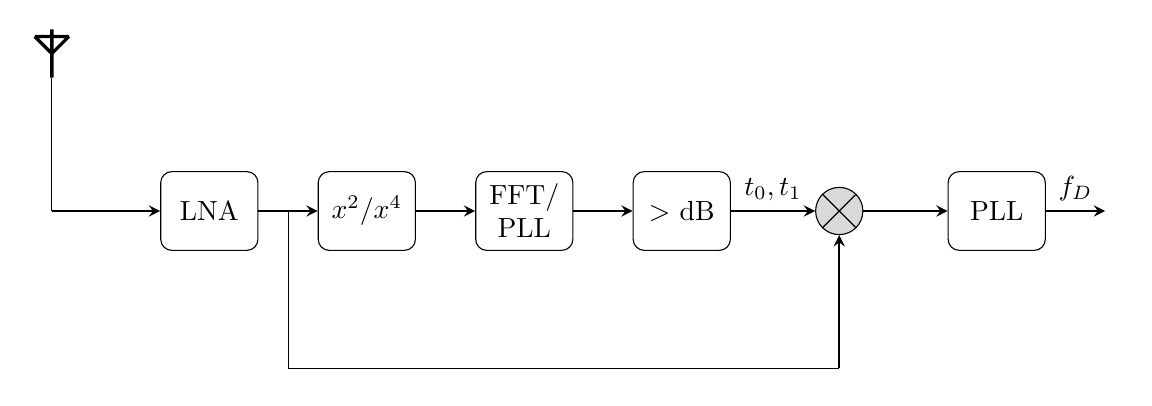
\begin{tikzpicture}[node distance=2cm]

% Sum shape
\node (ant) [empty]{};
\draw [very thick] (ant.north east) -- (ant.center)
      (ant.north west) -- (ant.center)
      (ant.north east) -- (ant.north west)
      (ant.north) -- (ant.south);
\node (antb) [below of=ant]{};
\node (lna) [block, right of=antb] {LNA};
\node (pwr) [block, right of=lna] {$x^2$/$x^4$};
\node (fft) [block, right of=pwr] {FFT/ PLL};
\node (thr) [block, right of=fft] {$>$ dB};
\node (sm1) [sum,   right of=thr]{};
\draw (sm1.north east) -- (sm1.south west)
      (sm1.north west) -- (sm1.south east);
\node (pll) [block, right of=sm1] {PLL};
\node (pllr)  [right of=sm1, xshift=1.5cm]{};

\draw (ant) -- (antb.center);
\draw [arrow] (antb.center) -- (lna);
\draw [arrow] (lna) -- (pwr) node[midway](bypass){};
\draw [arrow] (pwr) -- (fft);
\draw [arrow] (fft) -- (thr);
\draw [arrow] (thr) -- (sm1) node[midway,above]{$t_0, t_1$};
\draw [arrow] (sm1) -- (pll);
\node (sm1b) [below of=sm1]{};
\node (lnab) [below of=bypass]{};
\draw (bypass.center) -- (lnab.center);
\draw (lnab.center) -- (sm1b.center);
\draw [arrow] (sm1b.center) -- (sm1);
\draw [arrow] (pll) -- (pllr) node[midway,above]{$f_D$};
\end{tikzpicture}
\caption{General process of capturing a satellite signal}
\label{f_pos_tracking_block}
\end{figure}
% Zde, jako radioelektronik bych měl asi spoustu otázek. Ale lidi %mimo to nenapadne. Stejný obrázek 2.3 byl i v literatuře? Otázka %by byla, co tam dělá to násobení, a jestli PLL je skutečně %zavěšeno na tom signálu po kvadrátu, a zda je to skutečně PLL, %nebo i FLL. Mluvíte o těchto věcech někde dál? Pokud ne, mělo by %být zmíněno že tohle řeší už nějaký hotový SW. Ale citace %16,17,18 tam jsou, ok.
%% tohle je obecné, objevuje se to v několika zdrojích - pro můj kód je to v Designu


\section{Calculating satellite position}
\label{s_pos_tle_sgp4} 
The Doppler method requires the knowledge of the position of the transmitting satellite, which is then used as a reference. Unless the satellite itself transmits its position (which is the case for Iridium Ring Alert messages, albeit in a low resolution), the 
% to malé rozlišení - bude někde ještě zmíněn ten rozdíl co mezi ním a TLE od Noradu je, a jak jste na něj přišel?
%% je to ukázáno v Design
position needs to be calculated on the user side. To do this, the satellite orbit needs to be known and a propagation model used to calculate the satellite position at a given time.

A widely used approach utilises Two Line Element (TLE) sets, which contain orbital parameters for satellites, and the Simplified General Perturbations-4 (SGP4) model for propagation. TLEs are regularly updated by the North American Aerospace Defense Command (NORAD) and are publicly available via e.g. the CelesTrak project website\cite{des11}. An analysed example of TLE is shown in \autoref{f_pos_tle}. A TLE is valid for a given time, called an \textit{epoch}.

\begin{figure}
    \centering
    \includegraphics[width=1\linewidth]{img/pos_tle.PNG}
    \caption{Structure of a TLE set\cite{pos06}}
    \label{f_pos_tle}
\end{figure}

The SGP4 model is an orbit propagation model developed by the U.S. Air Force in the 1960s and further refined e.g. by Vallado et al.\cite{des06}. It is compatible with TLEs and commonly used together. The perturbation calculations are simplified - the Earth’s gravitational model is truncated, the atmospheric model is a static density field with exponential decay, and third-body influences are modelled only partially\citep{pos01}{698}. The SGP4 model works in the TEME coordinate frame (see \autoref{s_pos_frames_of_ref}).

The accuracy of the model was evaluated in \cite{pos07}, which concluded that for the satellite constellations under evaluation in this work the position prediction errors one day from TLE epoch are on the order of \qty{e2}{m}, with maximum errors between \qtyrange{3}{6}{km}, depending on the intensity of the Solar flux.



\section{Frames of reference}
\label{s_pos_frames_of_ref}
Any position needs to be expressed in a frame of reference. For terrestrial calculations, it is advantageous to use an Earth-centred frame, which has its origin at some centre (e.g. gravitational, physical) of the Earth. There are two general types of Earth-centred frames: Earth-Centred Inertial (ECI), which are fixed relative to some position external to the Earth (usually the Earth's position at equinox) and thus do not rotate with the Earth (they are inertial), and Earth-Centred Earth-Fixed (ECEF), which are fixed to a point on Earth and thus do rotate with it (they are non-inertial).

For this work, three frames of reference are important: TEME (ECI), ITRS (ECEF) and WGS84 geodetic datum (ECEF).

The process of transforming between those systems is described e.g. in \cite{pos01}, and the transformations used in this work are all based on the equations and algorithms provided there: from TEME to ITRS \citep{pos01}{231-233}, from ITRS to geodetic \citep{pos01}{174-179} and back \citep{pos01}{146}.

\subsection{True Equator Mean Equinox}
The True Equator Mean Equinox (TEME) reference frame is a Cartesian ECI frame. The z-axis points along the Celestial Ephemeris Pole\footnote{The Earth rotation axis} (CEP), while x-axis is located on the True Equator plane (a plane perpendicular to the CEP) and points in the direction of the Vernal Equinox without accounting for celestial nutation (the \textit{mean} or \textit{uniform} equinox)\citep{pos01}{231-233}. TEME frame is used by the SGP4 algorithm (see \autoref{s_pos_tle_sgp4}).

\subsection{International Terrestrial Reference System}
The International Terrestrial Reference System (ITRS) is a standard Cartesian ECEF frame. The origin is at the centre of mass of the Earth and the axes are fixed to defining coordinates on Earth. As a result of tectonic movement, the system is periodically recalculated\citep{pos01}{152}. All calculations within this work are done in ITRS.

\subsection{World Geodetic System Geodetic Datum}
The World Geodetic System-84 (WGS84), where 84 refers to the most recent version from 1984, is an ECEF frame maintained by the U.S. National Geospatial-Intelligence Agency. The WGS84 and ITRS agree on a level of \unit{cm}\citep{pos01}{203}. The geodetic datum  (hereafter referred to as only \textit{geodetic frame}) is a latitude-longitude-altitude ($\phi, \lambda, h$ respectively) frame defined within WGS84. In this work, the estimated position is in the geodetic frame for clarity, however, for navigation calculations themselves the position is always converted to ITRS.

% Opět, výborně.
%% Díky :)